\section{Gadgets}
\label{gadgets}


% { \tt Gadget}( $\left\langle \text{Input} \right\rangle, \left\langle \text{Output}  \right\rangle$ )

\newcommand{\warpunit}{{\tt Warp\_Unit}}
\newcommand{\prewarp}{{\tt Pre\_Warp}}
\newcommand{\firstwarp}{{\tt First\_Warp}}
\newcommand{\warpbridge}{{\tt Warp\_Bridge}}
\newcommand{\secondwarp}{{\tt Second\_Warp}}
\newcommand{\postwarp}{{\tt Post\_Warp}}

\newcommand{\dtop}{{\tt Digit\_Top}}
\newcommand{\dwriter}{{\tt Digit\_Writer}}
\newcommand{\dreader}{{\tt Digit\_Reader}}

\newcommand{\returnfromdonereadnextrow}{{\tt Return\_From\_Digit1\_Read\_Next\_Row}}
\newcommand{\returnfromdtworeadnextrow}{{\tt Return\_From\_Digit2\_Read\_Next\_Row}}
\newcommand{\returnfromdthreereadnextrow}{{\tt Return\_From\_Digit3\_Read\_Next\_Row}}

\newcommand{\returnfromdonereaddtwo}{{\tt Return\_From\_Digit1\_Read\_Digit2}}
\newcommand{\returnfromdonereaddtwocasetwo}{{\tt Return\_From\_Digit1\_Read\_Digit2\_Case2}}
\newcommand{\returnfromdtworeaddthree}{{\tt Return\_From\_Digit2\_Read\_Digit3}}
\newcommand{\returnfromdthreereaddone}{{\tt Return\_From\_Digit3\_Read\_Digit1}}

\newcommand{\inc}{{\tt carry}}

\newcommand{\dtopdonecaseone}{{\tt Digit\_Top\_Digit1\_Case1}}
\newcommand{\dtopdonecasetwo}{{\tt Digit\_Top\_Digit1\_Case2}}
\newcommand{\dtopdtwocasetwo}{{\tt Digit\_Top\_Digit2\_Case2}}
\newcommand{\dtopdthreecasethree}{{\tt Digit\_Top\_Digit3\_Case3}}

% todo: fix wording
When describing a special case, i.e. ``digit $x$ -- case $y$'', whatever follows
will only apply to the MSR (due to each case only affecting the MSR.)

\subsection{ Counter Unit }



    \subsubsection{ Digit readers }

    % For each digit length L
    \subsubsection{ Warping }

    % For each index in 1, 2, 3, and carry in 0,1
        For each $d \in \{0, 1\}^l$, $i = 1, 2, 3$

        \begin{enumerate}[label={--}]

            \item $\prewarp   (\langle d, i, \inc\rangle)$
                \begin{figure}[H]
                    \begin{subfigure}[t]{0.2\textwidth}
                        \centering
                        \includegraphics[width=0.2\textwidth]{warping/pre_warp_general}
                        \caption{\label{fig:warping/pre_warp_general} General }
                    \end{subfigure}%
                    ~
                    \begin{subfigure}[t]{0.2\textwidth}
                        \centering
                        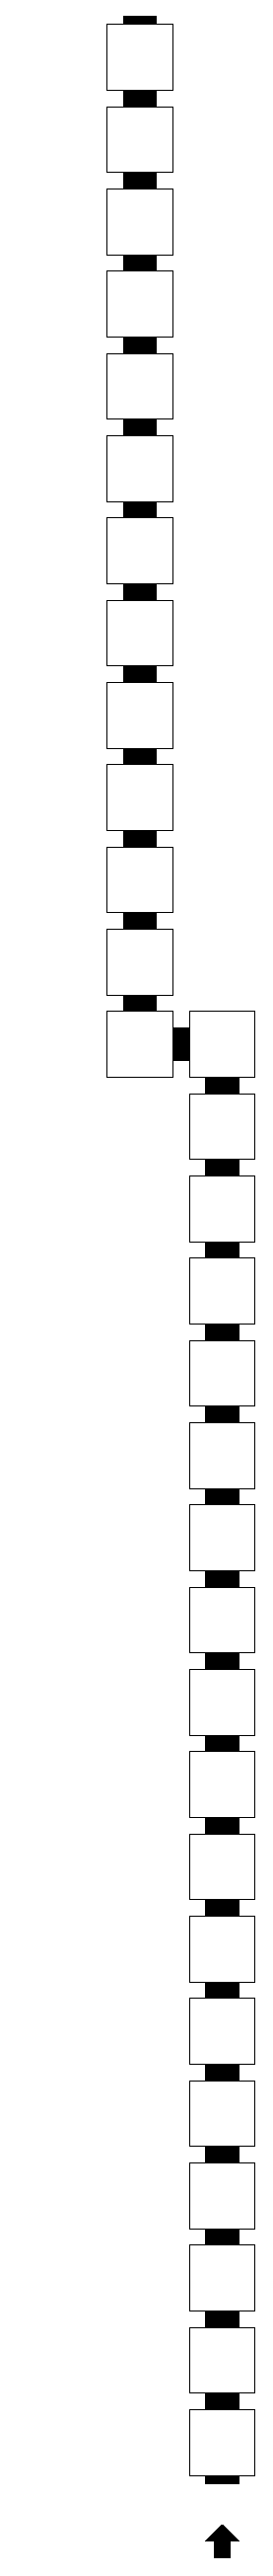
\includegraphics[width=0.2\textwidth]{warping/pre_warp_case1_digit1_msr}
                        \caption{\label{fig:warping/pre_warp_case1_digit1_msr} Digit 1 -- Case 1}
                    \end{subfigure}%
                    ~
                    \begin{subfigure}[t]{0.2\textwidth}
                        \centering
                        \includegraphics[width=0.2\textwidth]{warping/pre_warp_case2_digit1_msr}
                        \caption{\label{fig:warping/pre_warp_case2_digit1_msr} Digit 1 -- Case 2}
                    \end{subfigure}%
                    ~
                    \begin{subfigure}[t]{0.2\textwidth}
                        \centering
                        \includegraphics[width=0.2\textwidth]{warping/pre_warp_case2_digit2_msr}
                        \caption{\label{fig:warping/pre_warp_case2_digit2_msr} Digit 2 -- Case 2}
                    \end{subfigure}%
                    ~
                    \caption{\label{fig:pre_warp_gadgets} {\prewarp} gadgets }
                \end{figure}


            \item $\firstwarp (\langle d, i, \inc\rangle)$
                1 tile is created

            \item $\warpbridge(\langle d, i, \inc\rangle)$

                A {\warpbridge} gadget binds the last tile of the {\firstwarp} gadgets to the
                first tile of the {\secondwarp} gadgets. In case 1, and case 2 - digit 1, the
                {\warpbridge} is omitted from the {\warpunit}.

                \begin{figure}[H]
                    \begin{subfigure}[t]{0.2\textwidth}
                        \centering
                        \includegraphics[width=0.2\textwidth]{warping/warp_bridge_general}
                        \caption{\label{fig:warping/warp_bridge_general} General}
                    \end{subfigure}%
                    ~
                    \begin{subfigure}[t]{0.2\textwidth}
                        \centering
                        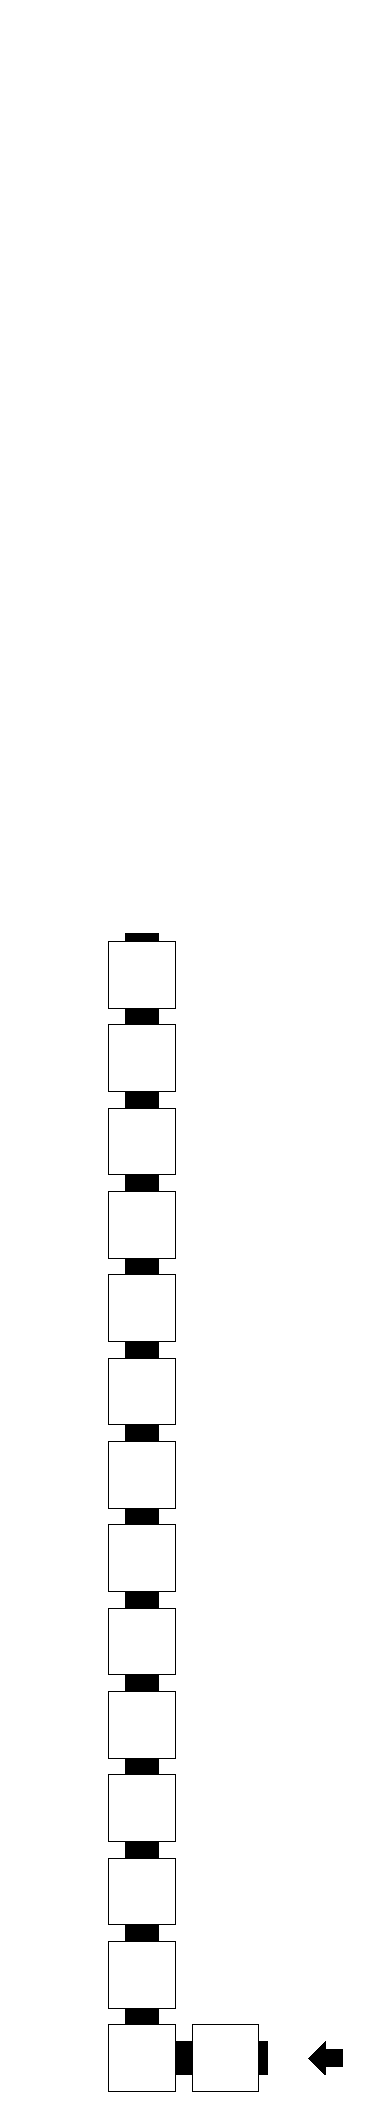
\includegraphics[width=0.2\textwidth]{warping/warp_bridge_case2_digit2_msr}
                        \caption{\label{fig:warping/warp_bridge_case2_digit2_msr} Digit 2 -- Case 2}
                    \end{subfigure}%
                    ~
                \end{figure}


            \item $\secondwarp(\langle d, i, \inc\rangle)$
                1 tile is created


            \item $\postwarp  (\langle d, i, \inc\rangle)$
                \begin{figure}[H]
                    \begin{subfigure}[t]{0.2\textwidth}
                        \centering
                        \includegraphics[width=0.2\textwidth]{warping/post_warp_general_digit1}
                        \caption{\label{fig:warping/post_warp_general_digit1} General Digit 1}
                    \end{subfigure}%
                    ~
                    \begin{subfigure}[t]{0.2\textwidth}
                        \centering
                        \includegraphics[width=0.2\textwidth]{warping/post_warp_general_digit2and3}
                        \caption{\label{fig:warping/post_warp_general_digit2and3} General Digits 2 and 3 }
                    \end{subfigure}%
                    ~
                    \begin{subfigure}[t]{0.2\textwidth}
                        \centering
                        \includegraphics[width=0.2\textwidth]{warping/post_warp_case1_digit1_msr}
                        \caption{\label{fig:warping/post_warp_case1_digit1_msr} Digit 1 -- Case 1}
                    \end{subfigure}%
                    ~
                    \begin{subfigure}[t]{0.2\textwidth}
                        \centering
                        \includegraphics[width=0.2\textwidth]{warping/post_warp_case2_digit1_msr}
                        \caption{\label{fig:warping/post_warp_case2_digit1_msr} Digit 1 -- Case 2}
                    \end{subfigure}%
                    ~

                    \begin{subfigure}[t]{0.2\textwidth}
                        \centering
                        \includegraphics[width=0.2\textwidth]{warping/post_warp_case2_digit2_msr}
                        \caption{\label{fig:warping/post_warp_case2_digit2_msr} Digit 2 -- Case 2}
                    \end{subfigure}%
                    ~
                    \caption{\label{fig:post_warp_gadgets} {\postwarp} gadgets }
                \end{figure}

        \end{enumerate}

    % For each digit length L
    \subsubsection{ Digit writers }
        % For each index in 1, 2, 3, and carry in 0,1
        %


    \subsubsection{ Digit tops }
        The {\dtop} gadgets have specific geometry, such that they allow {\firstwarp} and
        {\secondwarp} units to ``wake up" and end their warp journey. A {\dtop} is placed on
        the north end of a digit. These hold a increment/copy signal and the regional index
        of the next digit to read.
        \vspace{1cm}

        For each {\inc} $\in \{ {\tt increment, copy } \}$
        \begin{itemize}
            \item General digit tops common to all assemblies

            \begin{figure}[H]
                \centering
                \begin{subfigure}[t]{0.2\textwidth}
                    \centering
                    \includegraphics[width=0.2\textwidth]{warping/digit_top_general}
                    \caption{\label{fig:warping/digit_top_general} General }
                \end{subfigure}%
                ~
            \end{figure}

            \begin{enumerate}[label={--}]
                \item Create
                $\begin{aligned}[t]
                    \dtop(& \left \langle \text{``DigitTopDigit1"}, l, \inc \right\rangle, & \\
                          & \left \langle \text{``ReturnD1ReadD2"},    \inc \right\rangle \;)
                \end{aligned}$
                \vspace{.5cm}

                \item Create
                $\begin{aligned}[t]
                    \dtop(& \left \langle \text{``DigitTopDigit2"}, l, \inc \right\rangle, & \\
                          & \left \langle \text{``ReturnD2ReadD3"},    \inc \right\rangle \;)
                \end{aligned}$
                \vspace{.5cm}

                \item Create
                $\begin{aligned}[t]
                    \dtop(& \left \langle \text{``DigitTopDigit3"}, l, \inc \right\rangle,  \\
                          & \left \langle \text{``ReturnD3ReadD1"},    \inc \right\rangle \;)
                \end{aligned}$

            \end{enumerate}


            \item MSR-specific digit tops. The first tile placed in all digit top gadgets is the rightmost, bottommost tile.

            \begin{figure}[H]
                \centering
                \begin{subfigure}[t]{0.2\textwidth}
                    \centering
                    \includegraphics[width=0.2\textwidth]{warping/digit_top_case1_digit1_msr}
                    \caption{\label{fig:warping/digit_top_case1_digit1_msr} Digit 1 -- Case 1}
                \end{subfigure}%
                ~
                \begin{subfigure}[t]{0.2\textwidth}
                    \centering
                    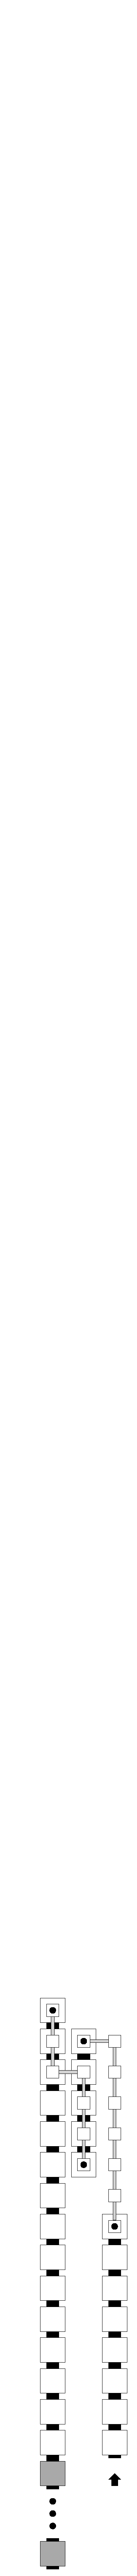
\includegraphics[width=0.2\textwidth]{warping/digit_top_case2_digit1_msr}
                    \caption{\label{fig:warping/digit_top_case2_digit1_msr} Digit 1 -- Case 2}
                \end{subfigure}%
                ~
                \begin{subfigure}[t]{0.2\textwidth}
                    \centering
                    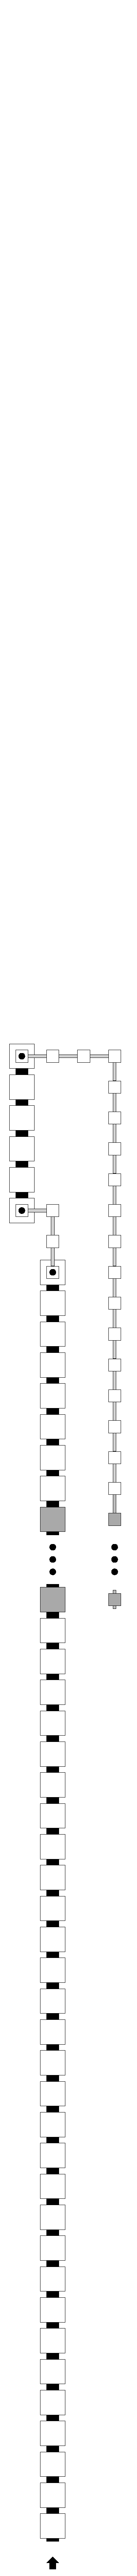
\includegraphics[width=0.2\textwidth]{warping/digit_top_case2_digit2_msr}
                    \caption{\label{fig:warping/digit_top_case2_digit2_msr} Digit 2 -- Case 2}
                \end{subfigure}%
                ~
                \begin{subfigure}[t]{0.2\textwidth}
                    \centering
                    \includegraphics[width=0.2\textwidth]{warping/digit_top_general}
                    \caption{\label{fig:warping/digit_top_general} Digit 3 -- Case 3}
                \end{subfigure}%
            \end{figure}


            \begin{itemize}
                % For digit 1, case 1
                \item if $i$ is 1 and MSR contains 1 digit and $l$ starts with 11:

                Create
                $\begin{aligned}[t]
                    \dtopdonecaseone(& \left \langle \text{``DigitTopDigit1--Case1"}, l, \inc \right\rangle, & \\
                                     & \left \langle \text{``ReturnD1ReadNextRow"},      \inc \right\rangle \;)
                \end{aligned}$
                \vspace{.5cm}


                % For digit 1, case 2
                \item if $i$ is 1 and MSR contains 2 digits and $l$ starts with 01:

                Create
                $\begin{aligned}[t]
                    \dtopdonecasetwo(& \left \langle \text{``DigitTopDigit1--Case2"}, l, \inc \right\rangle, & \\
                                     & \left \langle \text{``ReturnD1ReadD2--Case2"},    \inc \right\rangle \;)
                \end{aligned}$
                \vspace{.5cm}


                % For digit 2, case 2
                \item if $i$ is 2 and MSR contains 2 digits and $l$ starts with 11:

                Create
                $\begin{aligned}[t]
                    \dtopdtwocasetwo(& \left \langle \text{``DigitTopDigit2--Case2"}, l, \inc \right\rangle, & \\
                                     & \left \langle \text{``ReturnD2ReadNextRow"},     \inc \right\rangle \;)
                \end{aligned}$
                \vspace{.5cm}


                % For digit 3, in case 3
                \item if $i$ is 3 and MSR contains 3 digits and $l$ starts with 11:

                Create
                $\begin{aligned}[t]
                    \dtopdthreecasethree(& \left \langle \text{``DigitTopDigit3--Case3"}, l, \inc \right\rangle, & \\
                                         & \left \langle \text{``ReturnD3ReadNextRow"},     \inc \right\rangle \;)
                \end{aligned}$
                \vspace{.5cm}


            \end{itemize}

        \end{itemize}
    \vspace{1cm}



    \subsubsection{Return paths between the MSD and LSD in different rows}
        The gadgets of this class hold a increment/copy signal.
        The height of these gadgets is dependent on $l$ and the width is dependent of $k$.
        These gadgets are used to begin reading the first digit in the following row, once
        the MSD has been read in the current row.
        \vspace{1cm}

        \noindent For each {\inc} $\in \{ {\tt increment, copy } \}$

        \begin{itemize}
            \item Create
            $\begin{aligned}[t]
                \returnfromdonereadnextrow(& \left \langle \text{``ReturnD1ReadNextRow", \inc}       \right\rangle, & \\
                                           & \left \langle \text{``DigitReader"}, \epsilon, 1, \inc \right\rangle \;)
            \end{aligned}$

            \item Create
            $\begin{aligned}[t]
                \returnfromdtworeadnextrow(& \left \langle \text{``ReturnD2ReadNextRow", \inc}      \right\rangle, & \\
                                           & \left \langle \text{``DigitReader"}, \epsilon, 1, \inc \right\rangle \;)
            \end{aligned}$

            \item Create
            $\begin{aligned}[t]
                \returnfromdthreereadnextrow(& \left \langle \text{``ReturnD3ReadNextRow", \inc}      \right\rangle, & \\
                                             & \left \langle \text{``DigitReader"}, \epsilon, 1, \inc \right\rangle \;)
            \end{aligned}$
        \end{itemize}
    \vspace{1cm}



    \subsubsection{Return paths between digits in the same row}
        The gadgets of this class hold a increment/copy signal and the regional index
        of the next digit to read. The height of these gadgets is dependent on $l$.
        These gadgets are used so that upon writing a digit, the counter
        is able to move back down to the next digit in the current row, and continue
        reading.
        \vspace{1cm}

        \begin{figure}[H]
            \centering
            \begin{subfigure}[t]{0.2\textwidth}
                \centering
                \includegraphics[width=0.2\textwidth]{return_paths/return_digit1_read_digit2_general}
                \caption{\label{fig:return_paths/return_digit1_read_digit2_general} Return digit 1 read digit 2}
            \end{subfigure}%
            ~
            \begin{subfigure}[t]{0.2\textwidth}
                \centering
                \includegraphics[width=0.2\textwidth]{return_paths/return_digit1_read_digit2_case2_msr}
                \caption{\label{fig:return_paths/return_digit1_read_digit2_case2_msr} Return digit 1 read digit 2 -- Case 2}
            \end{subfigure}%
            ~
            \begin{subfigure}[t]{0.2\textwidth}
                \centering
                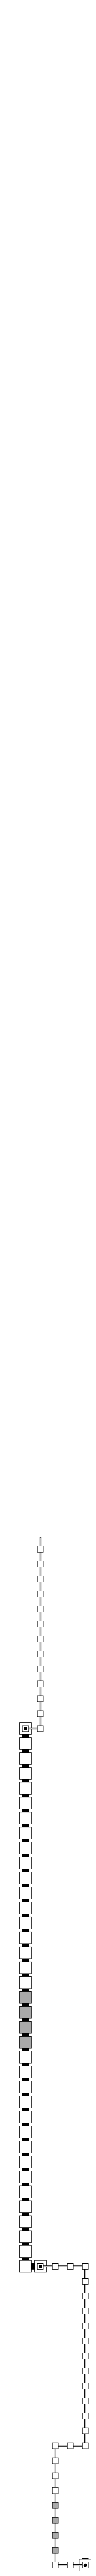
\includegraphics[width=0.2\textwidth]{return_paths/return_digit2_read_digit3_general}
                \caption{\label{fig:return_paths/return_digit2_read_digit3_general} Return digit 2 read digit 3}
            \end{subfigure}%
            ~
            \begin{subfigure}[t]{0.2\textwidth}
                \centering
                \includegraphics[width=0.2\textwidth]{return_paths/return_digit3_read_digit1_general}
                \caption{\label{fig:return_paths/return_digit1_read_digit2_general} Return digit 3 read digit 1}
            \end{subfigure}%
            \caption{\label{fig:return_path_same_row} All of these gadgets grow from north to south, the gray tiles have a height that
            depends on $l$.}
        \end{figure}

        \noindent For each {\inc} $\in \{ {\tt increment, copy } \}$.

        % todo yes/no?: pass L as input since gadget size is O(L), but inputs/outputs don't depend on it

        \begin{itemize}
            \item Create
            $\begin{aligned}[t]
                \returnfromdonereaddtwo(& \left \langle \text{``ReturnD1ReadD2"}, l, \inc,      \right\rangle, \\
                                        & \left \langle \text{``DigitReader"}, \epsilon, 2, \inc \right\rangle \;)
            \end{aligned}$

            \item Create
            $\begin{aligned}[t]
                \returnfromdonereaddtwocasetwo(& \left \langle \text{``ReturnD1ReadD2--Case2"}, l, \inc \right\rangle, \\
                                               & \left \langle \text{``DigitReader"}, \epsilon, 2, \inc \right\rangle \;)
            \end{aligned}$

            \item Create
            $\begin{aligned}[t]
                \returnfromdtworeaddthree(& \left \langle \text{``ReturnD2ReadD3"}, l, \inc        \right\rangle, \\
                                          & \left \langle \text{``DigitReader"}, \epsilon, 3, \inc \right\rangle \;)
            \end{aligned}$

            \item Create
            $\begin{aligned}[t]
                 \returnfromdthreereaddone(& \left \langle \text{``ReturnD3ReadD1"}, l, \inc       \right \rangle, \\
                                           & \left \langle \text{``DigitReader"}, \epsilon, 1, \inc \right \rangle \;)
            \end{aligned}$

        \end{itemize}

\subsection{Seed Unit}

